\documentclass[10pt,a4paper]{article}
\usepackage[utf8]{inputenc}
\usepackage{amsmath}
\usepackage{amsfonts}
\usepackage{amssymb}
\usepackage{graphicx}
\usepackage{fourier}
\author{José Jácome}
\begin{document}
%\chapter{Capitulo VII}
\section{TEORÍA DE SINGULARIDADES Y DEL RESIDUO.}
\subsection{SINGULARIDAD.-}
Un punto $z_0$ es un punto singular o una singularidad deu na función $F$, si $F$ es analítica en algún punto de toda variedad de $z_0$, excepto en $z_0$ mismo. \\
Existen Varios tipos de Singularidades.
\begin{enumerate}
\item[1º] \textbf{SINGULARIDAD AISLADA.-} El punto $z = z_0$ si $\exists \; \delta > 0$, tal que el círculo $\parallel z-z_0 \parallel= \delta$ no encierra puntos singulares distintos de $z_0$ (es decir $\exists \; V_{\delta} (z_0)$ sin singularidad). \\
Si tal $\delta \; \nexists $, decimos que $z_0$ es una singularidad no aislada. \\
Si $z_0$ no es un punto singular y si $\exists \; \delta > 0 \; / \; \parallel z - z_0 \parallel = \delta$ no encierra puntos singulares, decimos que $z_0$ es un punto ordinario de $F(z)$.
\item[2º] \textbf{POLOS.-} Si podemos encontrar un entero positivo $n$ tal que $\displaystyle{\lim_{ z \to z_0} (z-z_0)^n}$   \\$F(z) = A \neq 0$, entonces $z = z_0$ es llamado polo de orden $n$, si $n = 1$. $z_0$ es llamado un polo simple.\\
\textbf{Ejemplo.-} $f(z) = \dfrac{1}{(z-2)^3}$, se tiene un polo de orden tres en $z = 2$. \\
\textbf{Ejemplo.-} $f(z) = \dfrac{3 z - 2}{(z-1)^2(z+1)(z-4)}$;tiene un polo de orden dos en $z = 1$ y polos simples en $z = -1$ y $z = 4$\\
%pag 375
Si $y(z) = (z-z_0)^n F(z)$, de donde $F(z_0) \neq 0 $ y $n$ es un entero positivo, entonces $z = z_0$ es llamado un cero de orden $n$ de $y(z)$. \\
Si $n = 1$, $z_0$ es llamado un cero simple, en tal caso $z_0$ es un polo de orden $n$ de la función $\dfrac{1}{y(z)}$.
\item[3º] \textbf{LOS PUNTOS DE RAMIFICACIÓN.-} \\
\textbf{Ejemplos.-} \\
\begin{enumerate}
\item $\displaystyle{f(z) = (z-3)^{\dfrac{1}{2}}}$ tiene un punto de ramificación en $z = 3$
\item $f(z) = ln (z^2 + z -2)$ tiene puntos de ramificación donde $z^2+z-2 = 0$, es decir $z = 1$, $z = -2$. 
\end{enumerate}
\item[4º] \textbf{SINGULARIDADES REMOVIBLES.-} El punto singular $z_0$ es llamado una singularidad removible de $F(z)$ si $\lim_{z \to z_0 f(z)}$ existe.\\
\textbf{Ejemplo.-} El punto singular $z = 0$, es una singularidad removible de \\ $f(z) =\dfrac{sen(z)}{z}$, puesto que $\displaystyle{\lim_{z \to z_0} \dfrac{sen (z)}{z} = 1}$.
\item[5º] \textbf{SINGULARIDADES ESENCIALES.-} Una singularidad que no sea polo, ni punto de ramificiación, ni singularidad removible es llamado una singularidad esencial.\\
\textbf{Ejemplo.-} $f(z) = e^{\dfrac{1}{z-1}}$, tiene una singularidad esencial en $z = 2$ se una función unívoca tiene una singularidad, entonces las singularidades es un polo o una singularidad esencial, por esta razón un polo es llamado algunas veces una singularidad evitable.\\
Equivalentemente $z = z_0$ es una singularidad esencial si no podemos encontrar algún positivo $n$ tal que: $\displaystyle{\lim_{z \to z_0} (z-z_0)^n f(z) = A \neq 0}$. \\ 
\item[6º] \textbf{SINGULARIDAD EN EL INFINITO.-} El tipo de singularidad de $f(z)$ en $z = \inf$ (el punto en el infinito) es el mismo como el de $f(\dfrac{1}{w})$ en $w = 0$.\\
\textbf{Ejemplo.-} La función $f(z) = z^3$ tiene como polo de tercer orden en $z = \inf$, ya que $f(\dfrac{1}{w}) = \dfrac{1}{w^3}$ tiene un polo de tercer orden en $w = 0$.\\
\textbf{Ejemplo.-} Localizar y clasificar las singularidades\\
\begin{itemize}
\item [1)] $f(z) = \dfrac{z}{(z^2 + 4)^2}$ \\
\begin{center}
\underline{\textbf{Desarrollo}}
\end{center}
$f(z) = \dfrac{z}{(z^2 + 4)^2}$\\
$\displaystyle{\lim_{z \to 2 i} (z-2 i)^2 f(z) = \lim_{z \to 2 i} \dfrac{z}{(z + 2i)^2} = \dfrac{1}{8i} \neq 0}$, de donde $z = 2 i$ es un polo de segundo orden, simultánmeamente. \\
$z = -2i$ es un polo de segundo orden.  \\
Como se pueden encontrar $\delta \; > 0$ tal que ninguna singularidad distinta de $z = 2i$ está dentro del círculo. \\
$\parallel z - 2i \parallel = \delta$ entonces $z = 2i$ es una singularidad aislada, simultáneamente para $z = -2i$ es una singularidad aislada. 
\item[2)] $f(z) = \dfrac{ln(z-2)}{(z^2+2z+2)^2}$ \\
\begin{center}
\underline{\textbf{Desarrollo}}
\end{center}
El punto $z = 2$ es un punto de ramificación y es una singularidad aislada, también $z^2+2z+2 = 0$ de donde se tiene $z = -1 +- 2i$ y se dice que $z = -1 +- 2i$ son polos de cuarto orden de los culaes son singularidades aisladas. 
\item[3)] $f(z) = \dfrac{sen(\sqrt{z})}{\sqrt{z}}$ 
\begin{center}
\underline{\textbf{Desarrollo}}
\end{center}
Como $\displaystyle{\lim_{z \to 0} f(z) = \lim_{z \to 0} \dfrac{sen(\sqrt{z})}{\sqrt{z}} = 1 \neq 0}$, entonces $z = 0$ es una singularidad removible.

\end{itemize}
\end{enumerate}
\subsection{RESIDUOUS.-} 
Se conoce por el desarrollo de la serie de Laurent de una función analítica $f(z)$ es una región anular $D = \{ \; z\; \epsilon \; C \; R_1 < \parallel z - z_0 \parallel < R_2 \;\}  $ está dado por: \\
\begin{center}
$\displaystyle{f(z) = \sum_{n = 0}^{\infty} a_n (z-z_0)^n + \sum_{n = 1}^{\infty} b_n (z-z_0)^{-n}}$                                  ... (*)
\end{center}
Si la parte principial consiste de un número finito de términos es decir $b_n = 0$, para $n>m$ y $b_m \neq 0$ entonces la serie (*) toma la forma: \\
\begin{center}
$\displaystyle{f(z) = \sum_{n = 0}^{\infty} a_n (z-z_0)^n + \dfrac{b1}{z-z_0} + \dfrac{b2}{(z-z_0)^2} + .... + \dfrac{b_m}{(z-z_0)^m}+0+0...}$               
\end{center}
en este caso $F(z)$ tiene un polo de orden $m$ en $z=z_0$ y el coeficiente $b_1$ denotado por $a_{-1} = b_1$ recibe el nombre de residuo de $F$ en $z_0$. \\
Si $F(z)$ tiene un polo simple $z = z_0$, entonces la serie es $\displaystyle{f(z) = \sum_{n = 0}^{\infty} a_n (z-z_0)^n + \dfrac{b1}{z-z_0}}$\\
$\displaystyle{f(z) = a_0 + a_1(z-z_0) + a_2(z-z_0)^2 + ... + a_n(z-z_0)^n + ... + \dfrac{b_1}{z - z_0}}$ \\ 
$\displaystyle{(z-z_0)f(z) = a_0(z-z_0) + a_1(z-z_0)^2 + ...+ a_n(z-z_0)^{n+1} + ... + b_1}$ ahora tomamos el límite cuando $z \to z_0$ \\
se tiene: $\displaystyle{\lim_{z \to z_0} (z-z_0)f(z) = b_1=Re(f,z_0)}$ , $b_1$ recibe el nombre de $F(z)$ en $z = z_0$. \\                             
Luego si $F(z)$ tiene un polo en $z = z_0$ y $z_0$ est aen el interior de $\gamma$ entonces $\displaystyle{\oint_{\gamma} F(z)dz \neq 0}$ 
\begin{center}
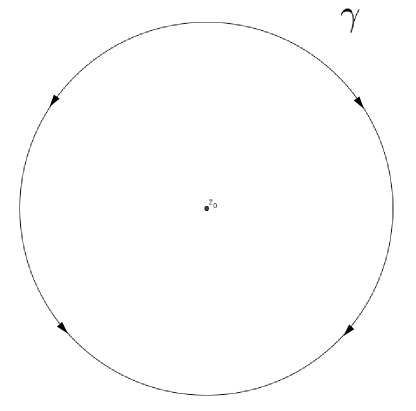
\includegraphics[scale=0.25]{1.png}
\end{center}
En este caso $F(z)$ se puede expresar mediante la serie \\
$\displaystyle{F(z) = \sum_{n = 0}^{\infty} a_n(z-z_0)^n + \sum_{n = 1}^{\infty} b_n(z-z_0)^n}$ , convergente $\forall \; z \; \epsilon \; C$ tal que \\
$\displaystyle{0 < \parallel z - z_0 \parallel < R}$ y $\displaystyle{a_n = \dfrac{1}{2 \pi i } \oint_{\gamma} \dfrac{F(z)dz}{(z-z_0)^{n+1}}}$ , $\displaystyle {b_n = \dfrac{1}{2 \pi i } \oint_{\gamma} F(z) dz}$ \\
donde $\gamma$ es una curva cerrada contenida e nel anillo $0 < \parallel z - z_0 \parallel < R$ \\
Si $n = 1$, $\displaystyle {b_1= \dfrac{1}{2 \pi i} \oint_{\gamma} F(z) dz}$, de donde \\
$\displaystyle{\oint_{\gamma} F(z)dz = 2 \pi b_1 i}$ donde $b_1$ es el coeficiente de $\dfrac{1}{z-z_0}$ y $b_1$ es el residuo de $F(z)$ que denotaremos por $Re(F,z_0) = b_1$, por lo tanto\\
\begin{center}
$\displaystyle{\oint_{\gamma} F(z)dz = 2 \pi i b_1 = 2 \pi i Re(F,z_0)}$\\
%%Ejemplo 1 y 2
\end{center}
\subsection{TEOREMA DEL RESIDUO.-}
Si $f(z)$ es uan fracción analítica dentror y sobre la curva $\gamma$ excepto en un número finito de puntos singulares $z_1,z_2,z_3,...,z_j,...,z_m$ pertenecientes al interior de $\gamma$, entonces: \\
\begin{center}
$\displaystyle{\oint f(z)dz = 2 \pi i \sum_{j = 1}^m Re(f,z_j)}$
\end{center}
\begin{center}
\textbf{\underline{Demostración}}
\end{center}
\end{document}